\section{Data Stores and Consistency}
\label{sec:store-consistency}

The abstract machine of Fig.~\ref{fig:txnimp} allows operations to
witness arbitrary subsets of the global state, thus assuming the
semantics of an eventually consistent ({\sc ec}) data
store\footnote{{\sc ec} guarantees that in the absence of further
updates, all reads witness the same global state \emph{eventually}. In
any finite trace, however, there are no guarantees on what a read
witnesses.}. There are however stores, such as relational databases,
that provide stronger consistency guarantees than {\sc ec}. Like the
isolation levels of transactions, the consistency level of the
underlying store also affects the semantics of a program in
non-trivial ways. In this section, we demonstrate how the semantics of
stronger stores with on-demand weak isolation can be captured in our
operational model so that we can use the reasoning framework developed
in \S\ref{sec:reasoning} to reason about such stores.

% A non-trivial $\I$ composed of isolation specifications from
% Fig.~\ref{fig:ansi-isolation} induces the machine to provide
% non-trivial isolation guarantees for transactions. However, weak
% isolation levels often only constrain the visibility sets of
% operations by dictating what \emph{not} to see; not what to see.  For
% instance, \iso{Repeatable Read} isolation prohibits operations of a
% transaction from witnessing different states. It, however, does not
% prohibit all operations of a transaction from witnessing an aribitrary
% subset of the global state. Consequently, the machine can remain an
% {\sc ec} store even while providing non-trivial isolation. How then to
% model the semantics of an {\sc sc} store, such as a relational
% database, with variable (weak) isolation?

Firstly, we observe that the semantics of stronger stores can be
captured by store-specific consistency constraints, along with
transaction-specific isolation constraints, via the trace invariant
$\I$. In particular, we split $\I$ into two components: (1).  $\I_s$,
the store-specific invariant, and (2). $\I_c$, the program-specific
(or, client-specific) invariant, to capture consistency and isolation
constraints, respectively. $\I$ is now a conjunction:
  $\I \,=\, \lambda\E.~\I_s(\E) \wedge \I_c(\E)$ (often simplified to
  $\I \,=\, \I_s\wedge\I_c$).
While the program-specific trace invariant ($\I_c$) and remains an
invariant regardless of the store, the store specific invariant
($\I_s$) changes from store to store depending on the consisteny
level. $\I_s$ for an {\sc ec} store is $true$. Stronger stores, such
as an {\sc sc} store, have non-trivial $\I_s$.

A strongly-consistent {\sc sc} store guarantees a total order of all
operations w.r.t $\visZ$ consistent with their chronological order. A
straightforward $\I_s$ for this store is the \C{SC} property
formalized below:
\begin{smathpar}
\begin{array}{l}
  \C{SC}(\E) \;=\; \forall\eta_1,\eta_2.~\{\eta_1,\eta_2\}
  \subseteq \E.\A \conj \id(\eta_1) < \id(\eta_2) \\
  \hspace*{2in}\Rightarrow \underE{\eta_1 \visar \eta_2}
\end{array}
\end{smathpar}
Unfortunately, $\I_s=\C{SC}$ conflicts with all isolation
specifications of Fig.~\ref{fig:ansi-isolation}. For instance,
consider a case where $\I_c(\E) \;=\; \forall
T_i.~\underE{\C{RC}(T_i)}$, a constraint that dictates all
transactions execute under \iso{Read Committed} isolation. Imagine a
sample execution where $\eta_1$'s transaction is not yet committed
when $\eta_2$ is generated. Letting $\eta_1$ be visible to $\eta_2$
violates $\I_c$, whereas not letting it be visible violates $\I_{s}$.
The only way to satisfy both the invariants is to rule out all the
executions that interleave the operations of one transaction with the
other, thereby enforcing serializability \footnote{Thus,
serializability is a natural generalization of {\sc sc} to
transactions.}. In general, when $\I_s$ is in conflict (but not
inconsistent) with $\I_c$, the only way to enforce both invariant sets
is to restrict concurrency. Clearly, this is unacceptable since it
defeats the very purpose of supporting weak isolation. 
% How then do we enforce weak isolation on a strongly consistent
% machine?

In practice, relational databases resolve the conflict by prioritizing
weak isolation (thus, concurrency and performance) over strong
consistency, so the execution traces do not necessarily satisfy {\sc
sc}. In particular, visibility constraints imposed by {\sc sc} are
violated if (and only if) they are found to be in conflict with the
constraints imposed by the isolation level. In the context of
aforementioned example, $\eta_1$ is not made visible to $\eta_2$
because doing so would violate $\I_c$. However, if $\I_c$ is true,
then the store makes $\eta_1$ visible to $\eta_2$ to honor its
consistency commitment\footnote{The term \emph{recency
commitment}~\cite{bailisvldb} is often used in practice, perhaps to
capture the best-effort nature of {\sc sc}.}. We generalize this
approach to any $\I_s$ and $\I_c$ by defining a \emph{maximum
visiblity principle} to determine an acceptable weakening of $\I_s$ in
case of a conflict with $\I_c$.  The principle requires the weakened
consistency guarantee ($\I_s'$) of the store to enforce all visibility
relationships imposed by the actual consistency guarantee ($\I_s$),
unless enforcing such a relationship violates $\I_c$. 
% The formal definition of the principle is relegated
% to the supplementary in the interest of space, but it can be
% understood in the context of an {\sc sc} store, where it weakens the
% store invariant to the following:
Formally:
\begin{definition}
$\I_s' : \E \rightarrow \Prop$ is said to be a maximum visibility
weakening of $\I_s : \E \rightarrow \Prop$ if and only if:
\begin{itemize}
  \item $\I_s'$ is weaker than $\I_s$: 
      $\forall\E.~ \I_s(\E) \Rightarrow \I_s'(\E)$, and
  \item In every trace $\E$ that satisfies $\I_c$, and for every pair
  of effects $\eta_1$ and $\eta_2$ in $\E$, if $\I_s(\E)$ requires
  $\eta_1$ to be visible to $\eta_2$, then so does $\I_s'(\E)$ unless
  extending $\E$ with $\visZ(\eta_1,\eta_2)$ violates
  $\I_c$\footnote{\GK{ToDo: consider other well-formedness conditions
  on trace, such as acyclicity of $\visZ$ and $\soZ$. Are they needed
  (considering that the machine never violates them)? Encode the
  specifications in Z3 and make sure they are consistent.}}:
  \begin{smathpar}
  \begin{array}{l}
  \forall\E,\eta_1,\eta_2.~ \I_c(\E) \Rightarrow (\I_s(\E)
    \Rightarrow \underE{\eta_1 \visar \eta_2}) \Rightarrow \\
    \hspace*{0.5in}(\I_s'(\E) \Rightarrow \underE{\eta_1 \visar
    \eta_2} \disj \neg\I_c(\E\,\cup\,(\emptyset,\{(\eta_1,\eta_2)\})))
  \end{array}
  \end{smathpar}
\end{itemize}
\end{definition}
Applying this principle, we can weaken {\sc sc} to obtain the
following store trace invariant ($\I_s$) for an {\sc sc} store whose
isolation constraints are captured by $\I_c$:
\begin{smathpar}
\begin{array}{lcl}
\I_s(\E) & = & \forall \eta_1,\eta_2.\, \{\eta_1,\eta_2\},
    \subseteq \E.\A \conj \id(\eta_1) <
    \id(\eta_2) \\
    & & \hspace*{0.5in} \Rightarrow 
      \underE{\eta_1 \visar \eta_2} \disj \neg\I_c(\E
    \cup (\emptyset,\{(\eta_1,\eta_2)\}))\\
\end{array}
\end{smathpar}
$\I_s$ requires a trace $\E$ to satisfy the visibility constraints of
{\sc sc} except in cases where they are in conflict with $\I_c$.
Instantiating the parameter $\I$  with $\I_s \wedge \I_c$ in
Fig.~\ref{fig:txnimp} results in an operational semantics that
describes relational database-like stores.

Semantics of a causally consistent data
store~\cite{gotsmanpopl16,LBC16} can also be obtained: by defining
$\I_s$ to be the causal consistency ({\sc cc}) invariant that is
appropriately weakened to resolve conflicts with $\I_c$. Details are
relegated to the supplementary in the interest of space.

\begin{remark}
Note that the purpose of maximum visibility principle is to
rationalize the observed behaviour of databases in practice. In
particular, it is not intended to be a guiding principle to engineer
data stores.
\end{remark}

% \paragraph{A CC store} A causally consistent data store~\cite{gotsmanpopl16,LBC16}
% allows operations to only witness a causally consistent snapshot of the
% global state. The store-specific invariant obtained by weakening the
% {\sc cc} guarantee to account for conflicts with $\I_c$ is shown
% below (the original {\sc cc} does not contain the $\neg\I_c(\dots)$
% disjuncts): 
% \begin{smathpar}
% \begin{array}{lccl}
% \C{CC}(\E) & \;=\; &  & \forall \eta_1,\eta_2.\, 
%       \E \Vdash \eta_1 \soar \eta_2 \Rightarrow  \underE{\eta_1 \visar
%       \eta_2} \\
%     & & & \hspace*{0.6in}\disj \neg\I_c(\E \cup 
%                 (\emptyset,\{(\eta_1,\eta_2)\}))\\
%     &   & \wedge & \forall\eta_1,\eta_2,\eta_3.\,\underE{\eta_1 \visar
%       \eta_2} \conj \underE{\eta_2 \visoar \eta_3} \\
%     &   & &\hspace*{0.3in} \Rightarrow \underE{\eta_1 \visar \eta_3}
%       \disj \neg\I_c(\E \cup (\emptyset,\{(\eta_1,\eta_2)\}))\\
% \end{array}
% \end{smathpar}

% \noindent Instantiating the parameter $\I$  with $\I_s \wedge \I_c$ in
% Fig.~\ref{fig:txnimp} results in an operational semantics that admits
% violation of causal consistency if and only if the violation is
% inevitable to enforce $\I_c$.

\subsection{Weakly Consistent Replication}

\begin{figure}
\centering
\subcaptionbox {
  Replica model
  \label{fig:ec-theirs}
} [
  0.4\columnwidth
] {
  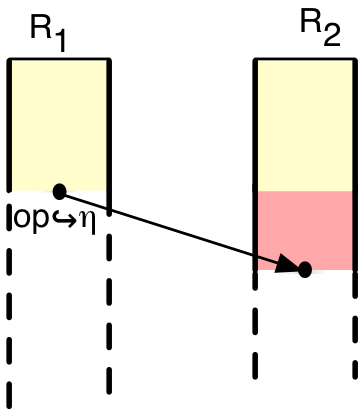
\includegraphics[scale=0.7]{Figures/ec-theirs}
 
}
\hspace*{0.1in}
\subcaptionbox {
  Subset model
  \label{fig:ec-ours}
}{
  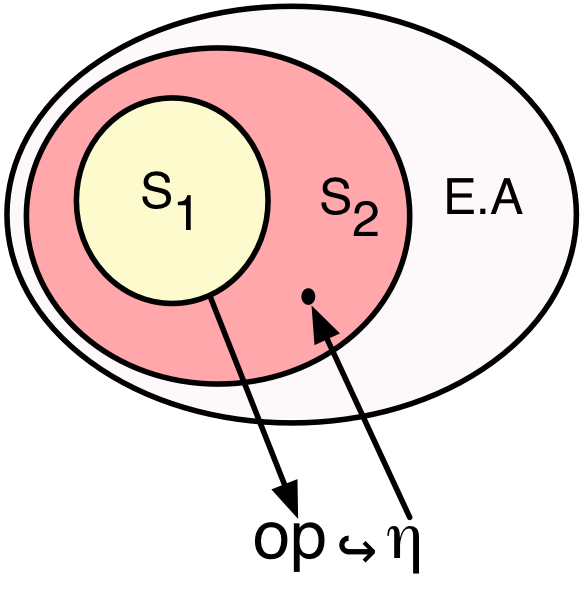
\includegraphics[scale=0.45]{Figures/ec-ours}
} \caption{In the replica model, operation $\op$ generates effect
$\eta$ at replica $R_1$, which is then merged to $R_2$. If the
\emph{store is {\sc cc}}, then $R_2$'s state at merge event is same or
larger than $R_1$'s state at generation event (the difference is
highlighted). In our subset model, $\op$ witnesses $S_1 \subseteq
\E.\A$ and generates $\eta$, which is immediately added to $\E.\A$. A
later operation may witness $S_2 \subseteq \E.\A$, and if the
\emph{operation is} {\sc cc} and $\eta \in S_2$, then it also
witnesses $S_1$ (i.e., $S_1 \subseteq S_2$). } 
% Moreover, Like $R_2 - R_1$, if all effects in $S_2 - S_1$ are
% concurrent with $\eta$, i.e., $\not\exists\eta'.~\eta' \in S_2 - S_1
% \conj % visZ(\eta,\eta')$, then any precondition $P$ that is valid
% when $\op$ executed is also valid when $\eta$ is witnessed because
% of the stability condition.
\label{fig:ec-theirs-vs-ours}
\end{figure}

Reasoning under weakly consistent replication has received special
attention in the recent work~\cite{gotsmanpopl16}. Our operational
semantics and proof system are general enough to admit replication as
a special case. In this section, we explain how the standard artifacts
of weakly consistent replication manifest in our reasoning framework.

Reasoning about weakly consistent replication often involves reasoning
in terms of \emph{replicas} of data. The primary challenge in this
setting is to ensure that the assumptions made and guarantees enforced
by an operation at one replica carry over to other replicas that merge
its effects, thus preserving the overall integrity of the system.
In~\cite{gotsmanpopl16}, this challenge is partly addressed by
imposing restrictions on how various replica states differ, i.e., by
fixing a system model with a stronger baseline consistency ({\sc cc})
than {\sc ec}. This unfortunately restricts the reasoning approach
from being applied to weaker stores such as Bayou~\cite{bayou} or
Quelea~\cite{pldi15}. Our view of replication however does not
explicitly involve replicas.  Fig.~\ref{fig:ec-theirs-vs-ours}
contrasts our model of weakly consistent replication with the
conventional replica-based model.  Under our model, the notion of a
replica is subsumed by the concept of visibility; a replica is defined
by the subset ($S$) of global state ($\E.\A$) that an operation
witnesses. Constraints over replica states therefore manifest as
constraints over the visibility relation.  For example, instead of
requiring the store to be causally consistent, an operation can
request to witness a causally consistent subset of the state; such
demands can be made via the trace invariant $\I$. For a precondition
($P$) of the operation to be useful, it has to be an assertion over
every causally consistent subset of the global state.  Since any
replica that eventually executes the operation has to expose one such
subset ($S$), the precondition is guaranteed to hold regardless of the
replica. There is however one problem with this explanation; by
considering subsets of just one global state, it ignores the fact that
the global state (hence, the replica states) change during the
execution of the operation. To account for this
change,~\cite{gotsmanpopl16} distinguishes between \emph{effect
generation} event at one replica and \emph{effect merge} event at
another replica, and requires that certain invariants be preserved
between these two events at different replicas. Our framework folds
all of this into a stability condition (\S\ref{sec:rely-guarantee}).
Since any change to the global state during the execution of the
operation is an interference, and $P$ is required to be stable with
respect to any such interference, it follows that $P$ is valid on
every replica, thus ensuring that assumptions made at the generation
event are also valid at the merge event.

\subsection{Example}


\begin{figure}
\centering
\begin{txnimpcode}
 $\begin{decoration}
 P_1:\{ {\neg\committed(\C{Wd2})} \Rightarrow \C{C = k} \conj\\
        \hspace*{0.3in}{\committed(\C{Wd2})} \Rightarrow \C{Wd2}
        \hboar \C{Wd1} \wedge \C{Wd2} \wrstoar \C{C} \wedge \C{C = k-a2} \}
 \end{decoration}$
  txn$\langle$'Wd1'$\rangle${
   $\begin{decoration}
    \phi_1 : \{{\neg\committed(\C{Wd2})} \Rightarrow \C{C = k} \conj
      {\committed(\C{Wd2})} \Rightarrow \C{Wd2} \wrstoar \C{C} \conj\\
       \hspace*{0.3in}{\committed(\C{Wd2})} \wedge
        {\C{Wd2} \hboar \C{Wd1}} 
       \Rightarrow \C{C = k-a2} \}
    \end{decoration}$ 
    v1 = C
   $\begin{decoration}
    \phi_2 : \{{\neg\committed(\C{Wd2})} \Rightarrow \C{C = k} \wedge \C{v1 = k} \conj\\
       \hspace*{0.3in}{\committed(\C{Wd2})} \Rightarrow \C{Wd2} \wrstoar \C{C} \conj \\
       \hspace*{0.3in}{\committed(\C{Wd2})} \wedge
        {\C{Wd2} \hboar \C{Wd1}} 
       \Rightarrow \C{C = k-a2} \wedge \C{v1 = k-a2}\}
    \end{decoration}$ 
    if (v1 $\ge$ a1) {
      v2 = C;
     $\begin{decoration}
      \phi_3 : \{{\neg\committed(\C{Wd2})} \Rightarrow \C{C = k} \wedge \C{v2 = k} \conj\\
       \hspace*{0.3in}{\committed(\C{Wd2})} \Rightarrow \C{Wd2} \wrstoar \C{C} \conj \\
         \hspace*{0.3in}{\committed(\C{Wd2})} \wedge
          {\C{Wd2} \hboar \C{Wd1}} \Rightarrow \C{C = k-a2} \wedge \\
          \hspace*{1.9in}\C{v2 = k-a2}\}
      \end{decoration}$ 
      v3 = v2 - a1;
     $\begin{decoration}
      \phi_4 : \{{\neg\committed(\C{Wd2})} \Rightarrow \C{C = k} \wedge \C{v3 = k-a1} \conj\\
         \hspace*{0.3in}{\committed(\C{Wd2})} \Rightarrow \C{Wd2} \wrstoar \C{C} \conj \\
         \hspace*{0.3in}{\committed(\C{Wd2})} \wedge
          {\C{Wd2} \hboar \C{Wd1}} 
         \Rightarrow \C{C = k-a2} \wedge \\
         \hspace*{1.9in}\C{v3 = k-a2-a1}\}
      \end{decoration}$ 
      C := v3
     $\begin{decoration}
      \phi_5 : \{{\neg\committed(\C{Wd2})} \Rightarrow \C{C = k-a1}) 
                \conj\\
         \hspace*{0.3in}{\committed(\C{Wd2})} 
                \Rightarrow \C{C = k-a1-a2}\}
      \end{decoration}$ 
    }
  }
 $\begin{decoration}
  Q_1 : \{{\neg\committed(\C{Wd2})} \Rightarrow \C{C = k-a1}
            \conj \committed(\C{Wd1}) \conj\\
      \hspace*{0.12in}{\committed(\C{Wd2})} 
          \Rightarrow \C{C = k-a1-a2} \}
  \end{decoration}$ 
\end{txnimpcode}

\caption{`Wd1' transaction decorated with assertions}
\label{fig:wd1-decorated}
\end{figure}

The fully decorated implementation of transaction `Wd1' is shown in
Fig.~\ref{fig:wd1-decorated}. Decorated `Wd2' is similar. Assignment
statements are broken down and temporary local variables (\C{v1},
\C{v2} and \C{v3}) are introduced so as to separate shared variable
reads and writes.  Since we reason in terms of executions, all
assertions implicitly refer to the current execution (just as hoare
triples implicitly refer to the current state). Also implicit is the
invariant \C{k $\ge$ a1+a2}. Proposition $\committed(T)$ indicates
that the transaction $T$ is already committed. Precondition ($P_1$) of
`Wd1' accounts for the possibility of `Wd2' committing before `Wd1',
writing \C{k-a2} to \C{C}.  Precondition of `Wd2' is similar.  Since
neither `Wd1' nor `Wd2' are committed at the beginning, the
precondition in Fig.~\ref{fig:motiv-eg-1} is extended to include
$\neg\committed(\C{Wd1}) \wedge \neg\committed(\C{Wd2})$, from which
$P_1$ follows. Once the execution is inside `Wd1', commit of `Wd2'
($\committed(\C{Wd2})$) may mean that either `Wd2' happened before
`Wd1', or that it committed concurrently with `Wd1'. Since SI
proscribes the latter possibility, we only consider the case when
$\C{Wd2} \hboar \C{Wd1}$. A proof for $\C{Wd2} \hboar \C{Wd1}$ is
obtained subsequently, allowing us to get rid of the special case.

The first obligation is to show that the assertions that decorate
`Wd1' are indeed valid. This entails proving that, for each statement
of `Wd1', if evaluating the statement and extending an execution that
satisfies its precondition results in a well-formed execution, then
the extended execution must satisfy the postcondition. The
well-formedness assumption lets us ignore the executions that violate
the trace invariant lead the machine to a stuck state. This is useful
in case of the assignment statement that writes \C{v3} to \C{C}. Since
`Wd2' also writes to \C{C}, the trace invariant ($\I$) requires
$\C{Wd2} \hboar \C{Wd1}$ if $\committed(\C{Wd2})$ (the alternative
$\C{Wd1} \hboar \C{COMMIT}(\C{Wd2})$ allowed by \C{SI(Wd1)} is
impossible in this case because \C{Wd2} has already committed, while
\C{Wd1} is still in progress). This lets us treat the special case
$\committed(\C{Wd2})\conj \C{Wd2} \hboar \C{Wd1}$ as being equivalent
to the general case $\committed(\C{Wd2})$, which is required to prove
the postcondition of `Wd1'. Observe that \C{RC(Wd1)} does not justify
this generalization, hence replacing \C{SI(Wd1)} by \C{RC(Wd1)} is not
sufficient to prove the postcondition of `Wd1'.

The second obligation is to prove that assertions are valid despite
the interference from the the concurrent thread executing `Wd2'. The
interference is given by the following rely relation ($R_1$):
\begin{smathpar}
\begin{array}{lcl}
  R_1 & = & \{ (\E,\E') \;|\; \neg\underE{\committed(\C{Wd2})} \conj 
        \underE{\I} \conj \E'\Vdash \I \conj\\
%       \conj (\E'-\E) \subseteq \C{Wd2} \conj \\
%   & & \hspace*{0.5in} \E' \Vdash \committed(\C{Wd2}) ~\Rightarrow~ \E'
%       \Vdash \C{Wd2} \wrstoar \C{C} \conj \\ 
%   & & \hspace*{0.5in} \underE{\committed(\C{Wd1})} \conj \E' \Vdash
%   \committed(\C{Wd2}) \Rightarrow \C{C=k-a1-a2} \\
    & & \hspace*{0.5in} \neg\underE{\committed(\C{Wd1})} \conj
        \C{COMMIT(Wd2)} \in (\E'-\E) \\
    & & \hspace*{0.8in}\Rightarrow \C{C=k-a2} \conj 
        \E' \Vdash \C{Wd2} \wrstoar \C{C} \conj \\
    & & \hspace*{0.5in} \underE{\committed(\C{Wd1})} \conj
        \C{COMMIT(Wd2)} \in (\E'-\E) \\
    & & \hspace*{0.6in}\Rightarrow \C{C=k-a1-a2} \conj
        \E' \Vdash \C{Wd2} \wrstoar \C{C} \}\\
\end{array}
\end{smathpar}
The rely relation says the following about the concurrent thread: (1).
It may interfere only if `Wd2' is not already committed, (2). Any
interference takes well-formed executions to well-formed executions,
(3). If the interference commits `Wd2', then `Wd2' should have already
written to \C{C}, and (4). The value written is either $\C{k-a1-a2}$
or $\C{k-a1}$ depending on whether or not `Wd1' has already committed.
Interference from `Wd2' is allowed between any two operations of
`Wd1', and assertions are required to be valid despite the
interference. For instance, if the execution ($\E$) immediately after
evaluating $\C{v1 = C}$ satisfies $\phi_2$ (i.e., $\underE{\phi_2}$),
and an interference from `Wd2' extends $\E$ to $\E'$ (i.e.,
$R_1(\E,\E')$), then the execution $\E'$ just before evaluating the
condition must satisfy $\phi_2$ (i.e., $\E' \Vdash \phi_2$). Indeed,
all $\phi_i$'s do satisfy this \emph{stability} condition, thus
lending the validity to the proof.
